\resizebox{0.95\textwidth}{!}{%
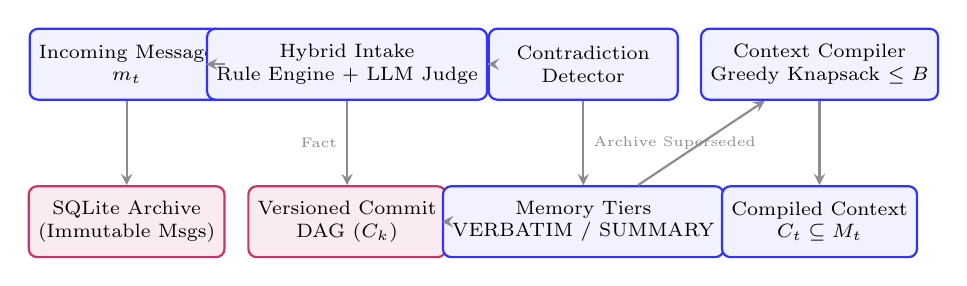
\begin{tikzpicture}[
    box/.style={rectangle, draw=blue!80, fill=blue!5, thick, rounded corners=3pt, minimum width=2.4cm, minimum height=0.9cm, align=center, font=\scriptsize},
    databox/.style={rectangle, draw=purple!80, fill=purple!8, thick, rounded corners=3pt, minimum width=2.4cm, minimum height=0.9cm, align=center, font=\scriptsize},
    flow/.style={->, >=stealth, thick, color=gray!90}]

\node[box] (msg) {Incoming Message\\$m_t$};
\node[box, right of=msg, xshift=1.8cm] (class) {Hybrid Intake\\Rule Engine + LLM Judge};
\node[databox, below of=msg, yshift=-1.0cm] (rawdb) {SQLite Archive\\(Immutable Msgs)};
\node[databox, right of=rawdb, xshift=1.8cm] (dag) {Versioned Commit\\DAG ($C_k$)};
\node[box, right of=class, xshift=2.0cm] (contra) {Contradiction\\Detector};
\node[box, right of=dag, xshift=2.0cm] (tiers) {Memory Tiers\\VERBATIM / SUMMARY};
\node[box, right of=contra, xshift=2.0cm] (compiler) {Context Compiler\\Greedy Knapsack $\le B$};
\node[box, below of=compiler, yshift=-1.0cm] (prompt) {Compiled Context\\$C_t \subseteq M_t$};

\draw[flow] (msg) -- (class);
\draw[flow] (msg) -- (rawdb);
\draw[flow] (class) -- node[left, font=\tiny]{Fact} (dag);
\draw[flow] (class) -- (contra);
\draw[flow] (contra) -- node[right, font=\tiny]{Archive Superseded} (tiers);
\draw[flow] (dag) -- (tiers);
\draw[flow] (tiers) -- (compiler);
\draw[flow] (compiler) -- (prompt);

\end{tikzpicture}%
}
